\chapter{Breadth-first search}
\label{chap:breadthfirst}

De tweede manier om een augmenting path te vinden in een graaf is de breadth-first search. Deze methode wordt ook gebruikt in het Edmonds-Karp algoritme, dit algoritme is een specifieke variant van het Ford-Fulkerson algoritme. Deze methode vindt het kortste pad van $s$ naar $t$. Het kortste pad is in dit geval gedefineert als het pad met het laagste aantal kanten.

Het breadth-first doorlopen van een graaf is niet anders dan dat dat bij een tree gebeurt, elk niveau wordt volledig doorzocht, voordat het algoritme naar het niveau daar onder gaat. Dit is te zien in figuur \ref{fig:breadthFirstTree}, de getallen op de knopen geven aan in welke volgorde de boom doorzocht wordt.

\begin{figure}[h]
 \centering
 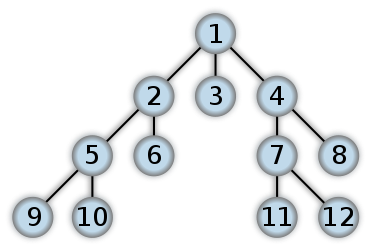
\includegraphics[width=0.5\linewidth]{breadthfirst/breadthfirsttree}
 \label{fig:breadthFirstTree}
 \caption{Breadth-first doorlopen van een boom}
\end{figure}

Om vervolgens het pad van $s$ naar $t$ te vinden in een graaf, wordt eerst de graaf doorlopen volgens het breadth-first principe totdat $t$ gevonden is. Terwijl de graaf doorlopen wordt, wordt bijgehouden welke kant leid naar welke knoop. Hierdoor is het gemakkelijk om het pad van $t$ naar $s$ terug te vinden. De pseudocode voor dit algoritme is te vinden in algoritme \ref{alg:breadthfirst}.

\section{Pseudocode}

\begin{algorithm}
 \caption{Breadth-first search path finding}
 \label{alg:breadthfirst}
 \begin{algorithmic}
  \REQUIRE \textbf{Input}: Graph G, Node s, Node t \\ 
\textbf{Output}: An augmenting path, or an empty path if none found.
  \STATE $Q \gets $ new queue
  \STATE $M \gets $ new hashmap
  \STATE $s$.state $\gets$ \textit{EXPLORED}
  \STATE $Q$.enqueue($s$)
  \WHILE{$\lnot Q$.isEmpty()}
   \STATE $v \gets Q$.dequeue()
   \FORALL{edge $e \in G$.incidentEdges($v$)}
    \IF{$e$.state = \textit{UNEXPLORED} $\land v$.residualCapacity() $ > 0$}
    \STATE $w \gets G$.opposite($v$, $e$)
    \IF{$\lnot w$.state = \textit{EXPLORED}}
      \STATE $Q$.enqueue($w$)
      \STATE $Q$.state = \textit{EXPLORED}
      \STATE $M$.put($w$, $e$) \COMMENT{$w$ discovered through edge $e$}
      \STATE $e$.state = \textit{DISCOVERY}
      \IF{$e$.start = $w$}
         \STATE Mark $e$ as forward
      \ELSE
         \STATE Mark $e$ as backward
      \ENDIF

      \IF{$w = t$}
         \STATE pathFound $\gets \FALSE$
         \STATE $p \gets w$
         \STATE $path \gets $ new list
         \WHILE{$\lnot$pathFound}
          \STATE $c \gets M$.get($p$) \COMMENT{Retreive edge $c$ that led to $p$}
          \STATE $path$.add($c$)      \COMMENT{Add edge $c$ to the path}
          \STATE $p \gets G$.opposite($p$, $c$) \COMMENT{ Go back another step in the graph}
          \IF{$p = s$}
            \STATE pathFound $\gets \TRUE$ \COMMENT{We found the start node, we are done.}
          \ENDIF
         \ENDWHILE
         \RETURN path
      \ENDIF
    \ENDIF
    \ELSE
      \STATE $e$.state $\gets$ \textit{BACKWARD}
    \ENDIF
   \ENDFOR
  \ENDWHILE
  \RETURN empty list \COMMENT{No path found}
 \end{algorithmic}
\end{algorithm}

\clearpage

\section{Analyse}
De grafen in \ref{fig:BFSgraph1} en \ref{fig:BFSgraph2} laten de uitkomst zien van het Ford-Fulkerson algoritme. De tabellen \ref{tbl:BFSgraph1} en \ref{tbl:BFSgraph2} geven de benchmarks weer voor de respectievelijke grafen.

\begin{table}[h]
 \begin{tabularx}{\linewidth}{| l | X |}
 \hline
 Maximale flow & 5 \\
 \hline
 Knopen bezocht & 11 \\
 \hline
 Kanten bezocht & 15 \\
 \hline
 Iteraties & 4 \\
 \hline
 Benodigde tijd & 57.061 ns \\
 \hline
\end{tabularx}
\centering
\caption{Resultaten voor graaf in figuur \ref{fig:BFSgraph1}}.
\label{tbl:BFSgraph1}
\end{table}

\begin{figure}[h]
	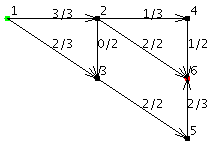
\includegraphics{breadthfirst/bfsgraph1}
	\centering
	\caption{Analyse van de eerste graaf}
	\label{fig:BFSgraph1}
\end{figure}

\begin{table}[h]
 \begin{tabularx}{\linewidth}{| l | X |}
 \hline
 Maximale flow & 7 \\
 \hline
 Knopen bezocht & 29 \\
 \hline
 Kanten bezocht & 48 \\
 \hline
 Iteraties & 7 \\
 \hline
 Benodigde tijd & 149.954 ns \\
 \hline
\end{tabularx}
\centering
\caption{Resultaten voor graaf in figuur \ref{fig:BFSgraph2}}.
\label{tbl:BFSgraph2}
\end{table}

\begin{figure}[h]
	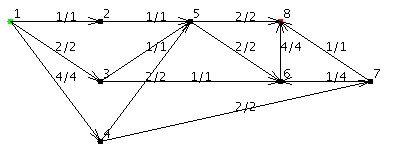
\includegraphics{breadthfirst/bfsgraph2}
	\centering
	\caption{Analyse van de tweede graaf}
	\label{fig:BFSgraph2}
\end{figure}